% questions.tex —— 2006 年·普通高等学校招生考试·重庆卷文科 · 题目内容片段（无答案）
% 由 tools/generate_projects.py 依来源总账自 2006/2006_数学真题_重庆文_试题.md 生成，勿手改（改源 MD 后重跑）


\begin{gktip}
\textbf{来源边界}：据固定候选 PDF 逐题转录，现场 SHA-256 与来源清单记录一致。题签支持卷名与科类的字面记录，但不能认证发布者、出版者、版次、扫描/重排来源链或官方原件身份。固定 PDF 仅见题面，未见答案、解析或评分标准，官方答案未录入。
\textbf{源页定位}：PDF 第 1 页（印刷页 286）含 Q1–Q19；第 2 页（印刷页 287）含 Q20–Q22。选择题 Q1–Q12，填空题 Q13–Q16，解答题 Q17–Q22。
\textbf{转录说明}：题面文字已与固定 PDF 原页逐题核对；文字层仅作定位候选。按原页保留字母、公式、条件与选项，不按题意推断修正。题图已依据固定候选 PDF 原页重绘为本卷 TikZ 源并链接；独立预览已检查，正式 TeX 构建与逐页视觉验收仍待完成。
\end{gktip}

\gkpart{一、选择题}

\begin{question}
\gkti{1}
已知集合 \(U=\{1,2,3,4,5,6,7\}\)，\(A=\{2,4,5,7\}\)，\(B=\{3,4,5\}\)，则 \((\complement_U A)\cup(\complement_U B)=\)（　）

(A) \(\{1,6\}\)　(B) \(\{4,5\}\)　(C) \(\{2,3,4,5,7\}\)　(D) \(\{1,2,3,6,7\}\)

\end{question}
\begin{question}
\gkti{2}
在等比数列 \(\{a_n\}\) 中，若 \(a_n>0\) 且 \(a_3a_7=64\)，则 \(a_5\) 的值为（　）

(A) 2　(B) 4　(C) 6　(D) 8

\end{question}
\begin{question}
\gkti{3}
以点 \((2,-1)\) 为圆心且与直线 \(3x-4y+5=0\) 相切的圆的方程为（　）

(A) \((x-2)^2+(y+1)^2=3\)　(B) \((x+2)^2+(y-1)^2=3\)

(C) \((x-2)^2+(y+1)^2=9\)　(D) \((x+2)^2+(y-1)^2=9\)

\end{question}
\begin{question}
\gkti{4}
若 \(P\) 是平面 \(\alpha\) 外一点，则下列命题正确的是（　）

(A) 过 \(P\) 只能作一条直线与平面 \(\alpha\) 相交

(B) 过 \(P\) 可作无数条直线与平面 \(\alpha\) 垂直

(C) 过 \(P\) 只能作一条直线与平面 \(\alpha\) 平行

(D) 过 \(P\) 可作无数条直线与平面 \(\alpha\) 平行

\end{question}
\begin{question}
\gkti{5}
\((2x-3)^5\) 的展开式中 \(x^2\) 项的系数为（　）

(A) \(-2160\)　(B) \(-1080\)　(C) \(1080\)　(D) \(2160\)

\end{question}
\begin{question}
\gkti{6}
设函数 \(y=f(x)\) 的反函数为 \(y=f^{-1}(x)\)，且 \(y=f(2x-1)\) 的图象过点 \(\left(\frac12,1\right)\)，则 \(y=f^{-1}(x)\) 的图象必过点（　）

(A) \(\left(\frac12,1\right)\)　(B) \(\left(1,\frac12\right)\)　(C) \((1,0)\)　(D) \((0,1)\)

\end{question}
\begin{question}
\gkti{7}
某地区有300家商店，其中大型商店有30家，中型商店有75家，小型商店有195家。为了掌握各商店的营业情况，要从中抽取一个容量为20的样本。若采用分层抽样的方法，抽取的中型商店数是（　）

(A) 2　(B) 3　(C) 5　(D) 13

\end{question}
\begin{question}
\gkti{8}
已知三点 \(A(2,3)\)，\(B(-1,-1)\)，\(C(6,k)\)，其中 \(k\) 为常数。若 \(|\overrightarrow{AB}|=|\overrightarrow{AC}|\)，则 \(\overrightarrow{AB}\) 与 \(\overrightarrow{AC}\) 的夹角为（　）

(A) \(\arccos\left(-\frac{24}{25}\right)\)

(B) \(\frac\pi2\) 或 \(\arccos\frac{24}{25}\)

(C) \(\arccos\frac{24}{25}\)

(D) \(\frac\pi2\) 或 \(\pi-\arccos\frac{24}{25}\)

\end{question}
\begin{question}
\gkti{9}
高三（一）班需要安排毕业晚会的4个音乐节目，2个舞蹈节目和1个曲艺节目的演出顺序，要求两个舞蹈节目不连排，则不同排法的种数是（　）

(A) 1800　(B) 3600　(C) 4320　(D) 5040

\end{question}
\begin{question}
\gkti{10}
若 \(\alpha,\beta\in\left(0,\frac\pi2\right)\)，\(\cos\left(\alpha-\frac\beta2\right)=\frac{\sqrt3}{2}\)，\(\sin\left(\frac\alpha2-\beta\right)=-\frac12\)，则 \(\cos(\alpha+\beta)\) 的值等于（　）

(A) \(-\frac{\sqrt3}{2}\)　(B) \(-\frac12\)　(C) \(\frac12\)　(D) \(\frac{\sqrt3}{2}\)

\end{question}
\begin{question}
\gkti{11}
设 \(A(x_1,y_1)\)，\(B\left(4,\frac95\right)\)，\(C(x_2,y_2)\) 是右焦点为 \(F\) 的椭圆 \(\frac{x^2}{25}+\frac{y^2}{9}=1\) 上三个不同的点，则“\(|AF|,|BF|,|CF|\) 成等差数列”是“\(x_1+x_2=8\)”的（　）

(A) 充要条件　(B) 必要而不充分条件

(C) 充分而不必要条件　(D) 既不充分也不必要条件

\end{question}
\begin{question}
\gkti{12}
若 \(a,b,c>0\) 且 \(a^2+2ab+2ac+4bc=12\)，则 \(a+b+c\) 的最小值是（　）

(A) \(2\sqrt3\)　(B) 3　(C) 2　(D) \(\sqrt3\)

\end{question}
\gkpart{二、填空题}

\begin{question}
\gkti{13}
已知 \(\sin\alpha=\frac{2\sqrt5}{5}\)，\(\frac\pi2<\alpha<\pi\)，则 \(\tan\alpha=\underline{\qquad\qquad}\)。

\end{question}
\begin{question}
\gkti{14}
在数列 \(\{a_n\}\) 中，若 \(a_1=1\)，\(a_{n+1}=a_n+2\)（\(n\geqslant1\)），则该数列的通项 \(a_n=\underline{\qquad\qquad}\)。

\end{question}
\begin{question}
\gkti{15}
设 \(a>0\)，\(a\ne1\)，函数 \(f(x)=\log_a(x^2-2x+3)\) 有最小值，则不等式 \(\log_a(x-1)>0\) 的解集为 \(\underline{\qquad\qquad}\)。

\end{question}
\begin{question}
\gkti{16}
\Needspace{5\baselineskip}
已知变量 \(x,y\) 满足约束条件
\nopagebreak[4]
\[
\begin{cases}
x+2y-3\leqslant0,\\
x+3y-3\geqslant0,\\
y-1\leqslant0,
\end{cases}
\]
若目标函数 \(z=ax+y\)（其中 \(a>0\)）仅在点 \((3,0)\) 处取得最大值，则 \(a\) 的取值范围为 \(\underline{\qquad\qquad}\)。

\end{question}
\gkpart{三、解答题}

\begin{question}
\gkti{17}
甲、乙、丙三人在同一办公室工作，办公室里只有一部电话机，设经该机打进的电话是打给甲、乙、丙的概率依次为 \(\frac16,\frac13,\frac12\)。若在一段时间内打进三个电话，且各个电话相互独立。求：

(1) 这三个电话是打给同一个人的概率；

(2) 这三个电话中恰有两个是打给甲的概率。

\end{question}
\begin{question}
\gkti{18}
设函数 \(f(x)=\sqrt3\cos^2\omega x+\sin\omega x\cos\omega x+a\)（其中 \(\omega>0, a\in\mathbb R\)），且 \(f(x)\) 的图象在 \(y\) 轴右侧的第一个最高点的横坐标为 \(\frac\pi6\)。

(1) 求 \(\omega\) 的值；

(2) 如果 \(f(x)\) 在区间 \(\left[-\frac\pi3,\frac{5\pi}6\right]\) 上的最小值为 \(\sqrt3\)，求 \(a\) 的值。

\end{question}
\begin{question}
\gkti{19}
设函数 \(f(x)=x^3-3ax^2+3bx\) 的图象与直线 \(12x+y-1=0\) 相切于点 \((1,-11)\)。

(1) 求 \(a,b\) 的值；

(2) 讨论函数 \(f(x)\) 的单调性。

\Needspace{0.4\textheight}
\end{question}
\begin{question}
\gkti{20}
如图，在正四棱柱 \(ABCD-A_1B_1C_1D_1\) 中，\(AB=1\)，\(BB_1=\sqrt3+1\)，\(E\) 为 \(BB_1\) 上使 \(B_1E=1\) 的点，平面 \(AEC_1\) 交 \(DD_1\) 于 \(F\)，交 \(A_1D_1\) 的延长线于 \(G\)。求：

(1) 异面直线 \(AD\) 与 \(C_1G\) 所成角的大小；

(2) 二面角 \(A-C_1G-A_1\) 的正切值。
\nopagebreak[4]
\begin{center}% Source-faithful schematic draft, not to scale.
% source_id=src-bfaf1f0ca2f3b8edd4a2455d39b464722513d2bb05efe36769938f1f187729e5
% source_sha256=fca2f5abda4a5e4982176417bf2f33b6b248847bffb0dcd09ae089c4f6a85b6e; PDF p.2; Q20.
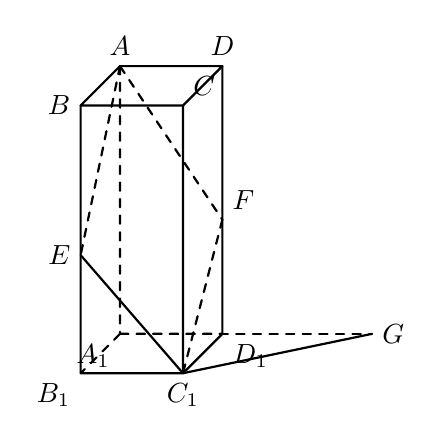
\begin{tikzpicture}[line cap=round,line join=round,thick]
  \coordinate (A) at (0,3.2); \coordinate (B) at (-0.5,2.7);
  \coordinate (C) at (0.8,2.7); \coordinate (D) at (1.3,3.2);
  \coordinate (A1) at (0,-0.2); \coordinate (B1) at (-0.5,-0.7);
  \coordinate (C1) at (0.8,-0.7); \coordinate (D1) at (1.3,-0.2);
  \coordinate (E) at (-0.5,0.8); \coordinate (F) at (1.3,1.25);
  \coordinate (G) at (3.2,-0.2);
  % Prism faces and edges. Rear/hidden edges are dashed as in the source.
  \draw (A)--(B)--(C)--(D)--cycle;
  \draw (B)--(B1) (C)--(C1) (D)--(D1) (B1)--(C1)--(D1);
  \draw[dashed] (A)--(A1) (A1)--(B1) (A1)--(D1);
  % E lies on BB1; plane A-E-C1-F meets DD1 at F.
  % G lies on the extension of A1-D1; C1-G is the requested line.
  \draw (E)--(C1) (C1)--(G);
  \draw[dashed] (A)--(E) (A)--(F) (F)--(C1);
  \draw[dashed] (A1)--(D1)--(G);
  \foreach \p/\pos/\lab in {A/above/A,B/left/B,C/above right/C,D/above/D,A1/below left/A_1,B1/below left/B_1,C1/below/C_1,D1/below right/D_1,E/left/E,F/above right/F,G/right/G}
    \node[\pos] at (\p) {$\lab$};
\end{tikzpicture}
\end{center}
\nopagebreak[4]
\end{question}
\begin{question}
\gkti{21}
已知定义域为 \(\mathbb R\) 的函数 \(f(x)=\frac{-2^x+b}{2^{x+1}+a}\) 是奇函数。

(1) 求 \(a,b\) 的值；

(2) 若对任意的 \(t\in\mathbb R\)，不等式 \(f(t^2-2t)+f(2t^2-k)<0\) 恒成立，求 \(k\) 的取值范围。

\Needspace{0.4\textheight}
\end{question}
\begin{question}
\gkti{22}
如图，对每个正整数 \(n\)，\(A_n(x_n,y_n)\) 是抛物线 \(x^2=4y\) 上的点，过焦点 \(F\) 的直线 \(FA_n\) 交抛物线于另一点 \(B_n(s_n,t_n)\)。

(1) 试证：\(x_ns_n=-4\)（\(n\geqslant1\)）；

\Needspace{5\baselineskip}
(2) 取 \(x_n=2^n\)，并记 \(C_n\) 为抛物线上分别以 \(A_n\) 与 \(B_n\) 为切点的两条切线的交点。试证：
\nopagebreak[4]
\[
|FC_1|+|FC_2|+\cdots+|FC_n|=2^n-2^{-n+1}+1.
\]
\nopagebreak[4]
\begin{center}% Source-faithful schematic draft. Coordinates satisfy x^2=4y exactly.
% source_id=src-bfaf1f0ca2f3b8edd4a2455d39b464722513d2bb05efe36769938f1f187729e5
% source_sha256=fca2f5abda4a5e4982176417bf2f33b6b248847bffb0dcd09ae089c4f6a85b6e; PDF p.2; Q22.
% Each pair has x_A*x_B=-4, so its chord passes through F=(0,1).
% Tangents use slope x/2; the A_n and B_n tangents meet at C_n.
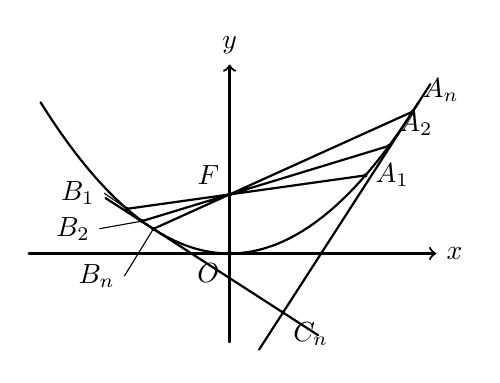
\begin{tikzpicture}[line cap=round,line join=round,thick,scale=0.75]
  \draw[->] (-3.4,0)--(3.5,0) node[right] {$x$};
  \draw[->] (0,-1.5)--(0,3.2) node[above] {$y$};
  \draw[domain=-3.2:3.2,samples=120] plot (\x,{\x*\x/4});
  \coordinate (O) at (0,0); \coordinate (F) at (0,1);
  \coordinate (A1) at (2.3,1.3225); \coordinate (B1) at (-1.73913,0.75614);
  \coordinate (A2) at (2.7,1.8225); \coordinate (B2) at (-1.48148,0.5487);
  \coordinate (An) at (3.1,2.4025); \coordinate (Bn) at (-1.29032,0.41623);
  \coordinate (Cn) at (0.90484,-1);
  % Focus chords A_i B_i, each passing through F.
  \draw (A1)--(B1) (A2)--(B2) (An)--(Bn);
  % Tangents at A_n and B_n: y=(x_n/2)x-x_n^2/4.
  \draw (0.5,-1.6275)--(An)--(3.4,2.8675);
  \draw (-2.1,0.9386)--(Bn)--(1.5,-1.3839);
  \fill (O) circle (1.2pt) node[below left] {$O$};
  \fill (F) circle (1.2pt) node[above left] {$F$};
  \foreach \p/\pos/\lab in {A1/right/A_1,A2/above right/A_2,An/above right/A_n,Cn/below right/C_n}
    \fill (\p) circle (1pt) node[\pos] {$\lab$};
  % Short leaders keep the three left labels distinct without moving points.
  \fill (B1) circle (1pt); \draw[thin] (B1)--(-2.12,1.02) node[left] {$B_1$};
  \fill (B2) circle (1pt); \draw[thin] (B2)--(-2.20,0.42) node[left] {$B_2$};
  \fill (Bn) circle (1pt); \draw[thin] (Bn)--(-1.78,-0.38) node[left] {$B_n$};
\end{tikzpicture}
\end{center}
\nopagebreak[4]

\end{question}